% -*- TeX -*- -*- UK -*- -*- Soft -*-

\chapter*{What this book is about}


Neural Networks and Deep Learning is a free online book \cite{Nielsen2015}. The book will teach you about: 
\begin{itemize}
\item  Neural networks, a beautiful biologically-inspired programming paradigm which enables a computer to learn from observational data 
\item Deep learning, a powerful set of techniques for learning in neural networks 
\end{itemize}

\section*{Historic View}


Vazquez2018

Favio V\'{a}zquez gives a brief introduction to Deep Learning \cite{Vazquez2018}\footnote{This blog post \cite{Vazquez2018} is well worth the read.}, with the following very  nice historic time line:

{\centering 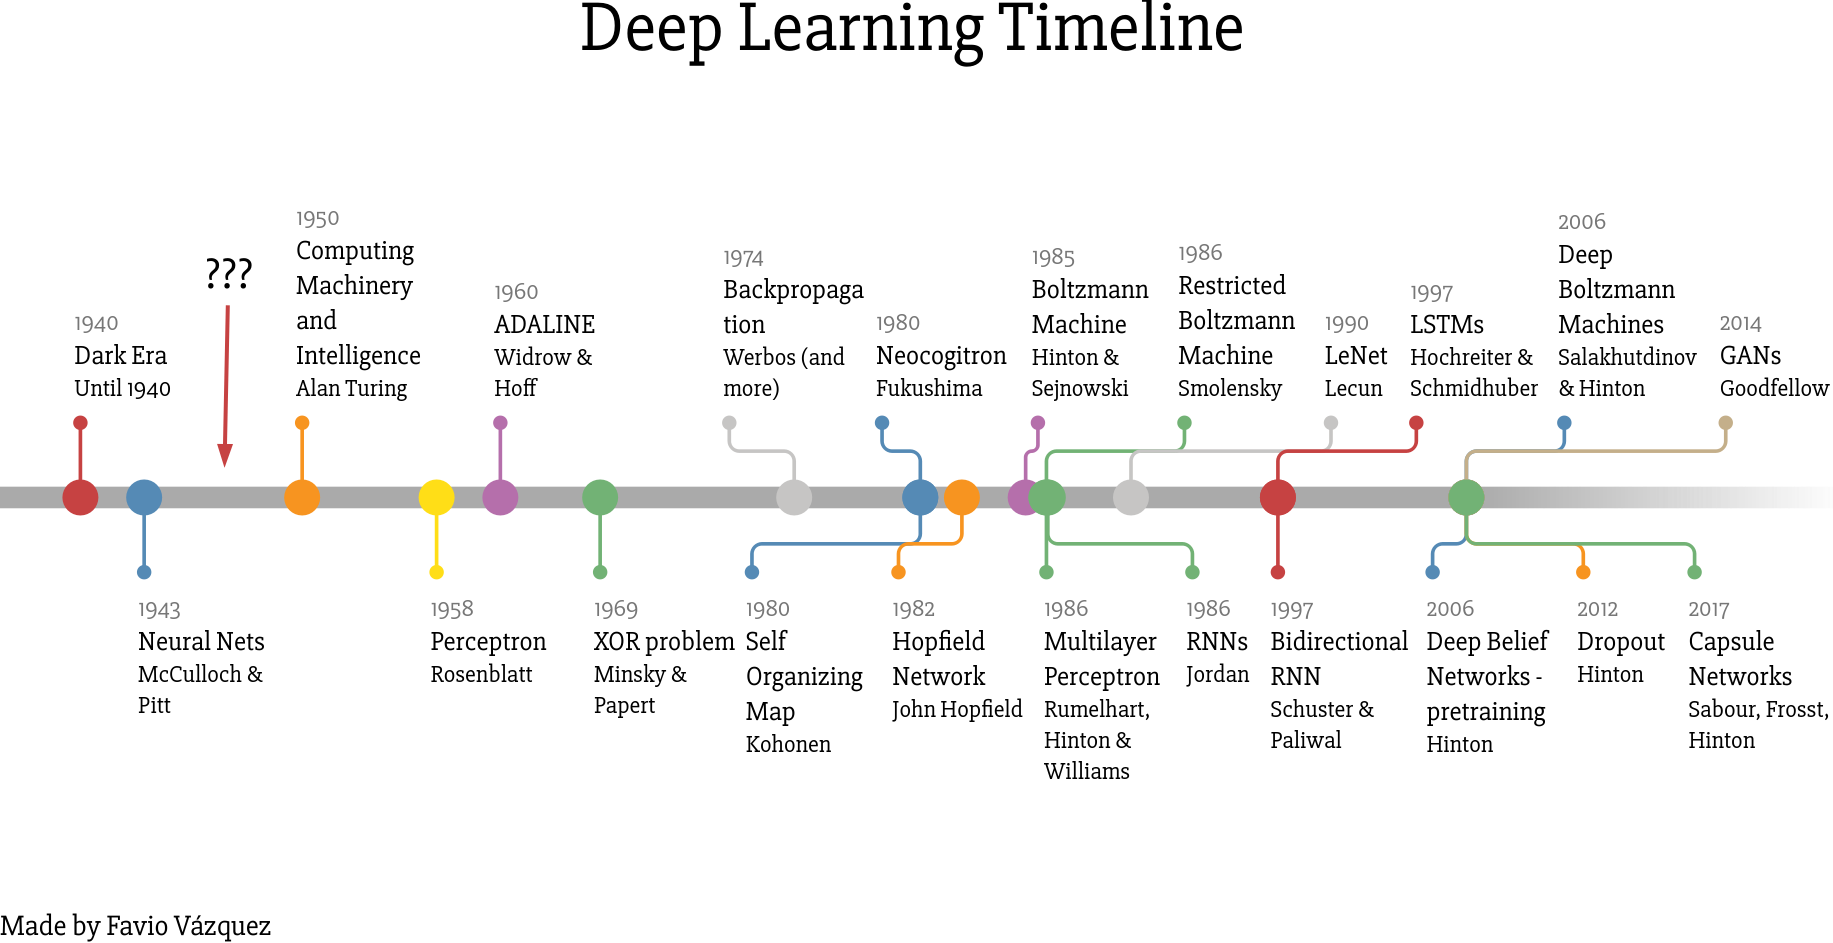
\includegraphics[width=\textwidth,]{pic/deeplearningtimeline.png} \par}

\section*{Overview}

Neural networks and deep learning currently provide the best solutions to many problems in image recognition, speech recognition, and natural language processing. This book will teach you many of the core concepts behind neural networks and deep learning. 

Neural networks are one of the most beautiful programming paradigms ever invented. In the conventional approach to programming, we tell the computer what to do, breaking big problems up into many small, precisely defined tasks that the computer can easily perform. By contrast, in a neural network we don't tell the computer how to solve our problem. Instead, it learns from observational data, figuring out its own solution to the problem at hand.

Automatically learning from data sounds promising. However, until 2006 we didn't know how to train neural networks to surpass more traditional approaches, except for a few specialized problems. What changed in 2006 was the discovery of techniques for learning in so-called deep neural networks. These techniques are now known as deep learning. They've been developed further, and today deep neural networks and deep learning achieve outstanding performance on many important problems in computer vision, speech recognition, and natural language processing. They're being deployed on a large scale by companies such as Google, Microsoft, and Facebook.

The purpose of this book is to help you master the core concepts of neural networks, including modern techniques for deep learning. After working through the book you will have written code that uses neural networks and deep learning to solve complex pattern recognition problems. And you will have a foundation to use neural networks and deep learning to attack problems of your own devising.

\section*{A principle-oriented approach}

One conviction underlying the book is that it's better to obtain a solid understanding of the core principles of neural networks and deep learning, rather than a hazy understanding of a long laundry list of ideas. If you've understood the core ideas well, you can rapidly understand other new material. In programming language terms, think of it as mastering the core syntax, libraries and data structures of a new language. You may still only ``know'' a tiny fraction of the total language - many languages have enormous standard libraries - but new libraries and data structures can be understood quickly and easily.

This means the book is emphatically not a tutorial in how to use some particular neural network library. If you mostly want to learn your way around a library, don't read this book! Find the library you wish to learn, and work through the tutorials and documentation. But be warned. While this has an immediate problem-solving payoff, if you want to understand what's really going on in neural networks, if you want insights that will still be relevant years from now, then it's not enough just to learn some hot library. You need to understand the durable, lasting insights underlying how neural networks work. Technologies come and technologies go, but insight is forever.

\section*{A hands-on approach}

We'll learn the core principles behind neural networks and deep learning by attacking a concrete problem: the problem of teaching a computer to recognize handwritten digits. This problem is extremely difficult to solve using the conventional approach to programming. And yet, as we'll see, it can be solved pretty well using a simple neural network, with just a few tens of lines of code, and no special libraries. What's more, we'll improve the program through many iterations, gradually incorporating more and more of the core ideas about neural networks and deep learning.

This hands-on approach means that you'll need some programming experience to read the book. But you don't need to be a professional programmer. I've written the code in Python (version 2.7\footnote{Some attempts will be made to convert these to Python 3, as will be documented in each case.}), which, even if you don't program in Python, should be easy to understand with just a little effort. Through the course of the book we will develop a little neural network library, which you can use to experiment and to build understanding. All the code is available for download from github \cite{Nielsengithub2019}. Once you've finished the book, or as you read it, you can easily pick up one of the more feature-complete neural network libraries intended for use in production.

On a related note, the mathematical requirements to read the book are modest. There is some mathematics in most chapters, but it's usually just elementary algebra and plots of functions, which I expect most readers will be okay with. I occasionally use more advanced mathematics, but have structured the material so you can follow even if some mathematical details elude you. The one chapter which uses heavier mathematics extensively is Chapter~\ref{sec:UsingNeuralNetsTorRcognizeHandWrittenDigits}, which requires a little multivariable calculus and linear algebra. If those aren't familiar, I begin Chapter~\ref{sec:UsingNeuralNetsTorRcognizeHandWrittenDigits} with a discussion of how to navigate the mathematics. If you're finding it really heavy going, you can simply skip to the summary of the chapter's main results. In any case, there's no need to worry about this at the outset.

It's rare for a book to aim to be both principle-oriented and hands-on. But I believe you'll learn best if we build out the fundamental ideas of neural networks. We'll develop living code, not just abstract theory, code which you can explore and extend. This way you'll understand the fundamentals, both in theory and practice, and be well set to add further to your knowledge.


\section*{On the exercises and problems}

It's not uncommon for technical books to include an admonition from the author that readers must do the exercises and problems. I always feel a little peculiar when I read such warnings. Will something bad happen to me if I don't do the exercises and problems? Of course not. I'll gain some time, but at the expense of depth of understanding. Sometimes that's worth it. Sometimes it's not.

So what's worth doing in this book? My advice is that you really should attempt most of the exercises, and you should aim \textit{not} to do most of the problems.

You should do most of the exercises because they're basic checks that you've understood the material. If you can't solve an exercise relatively easily, you've probably missed something fundamental. Of course, if you do get stuck on an occasional exercise, just move on --- chances are it's just a small misunderstanding on your part, or maybe I've worded something poorly. But if most exercises are a struggle, then you probably need to reread some earlier material.

The problems are another matter. They're more difficult than the exercises, and you'll likely struggle to solve some problems. That's annoying, but, of course, patience in the face of such frustration is the only way to truly understand and internalize a subject.

With that said, I don't recommend working through all the problems. What's even better is to find your own project. Maybe you want to use neural nets to classify your music collection. Or to predict stock prices. Or whatever. But find a project you care about. Then you can ignore the problems in the book, or use them simply as inspiration for work on your own project. Struggling with a project you care about will teach you far more than working through any number of set problems. Emotional commitment is a key to achieving mastery.

Of course, you may not have such a project in mind, at least up front. That's fine. Work through those problems you feel motivated to work on. And use the material in the book to help you search for ideas for creative personal projects.

\section*{Frequently Asked Questions}
\label{sec:FrequentlyAskedQuestions}

\begin{enumerate}

\item
Is there a pdf or print version of the book available, or planned? There's no pdf or print version available, nor planned.

\item
People sometimes suggest that it would be easy to convert the book to pdf or print. However, the book contains dozens of interactive JavaScript elements, and the narrative often depends on the reader interacting with those elements in some way. Doing the ``easy'' conversion would result in a poor quality product. Of course, those interactive parts could be rewritten to make sense in static form, but doing it well would be a big job.

\item
Can you help me with a mathematical problem, or with debugging my work? No. I suggest chatting about your problem with friends or colleagues. If that's no help, try an appropriate online forum to ask your question.

\item
Do you have solutions to the exercises and problems? Sorry, no.

\item
I'd like to do a translation into another language. Is that okay? It's fine under the terms of the book's license (see the page footer for details), provided: (1) you're not doing it for a product which is commercial in some way (e.g., you intend to sell it); and (2) you acknowledge me as the original author. I'd also appreciate a link, of course. If you have a commercial interest, please get in touch so we can discuss (mn@michaelnielsen.org).
\end{enumerate}

\section*{Acknowledgements}

The book grew out of a set of notes I prepared for an online study group on neural networks and deep learning. Many thanks to all the participants in that study group: Paul Bloore, Chris Dawson, Andrew Doherty, Ilya Grigorik, Alex Kosorukoff, Chris Olah, and Rob Spekkens. I learned a lot from all of you. I am particularly grateful to Rob, for providing so many insightful questions and ideas, and to Chris, who has continued to share his rapidly expanding knowledge of neural networks. Thanks also to Yoshua Bengio, who read and provided feedback on a chapter.

\section*{Attribution and License}

In academic work, please cite this book \cite{Nielsen2015} as: Michael A. Nielsen, ``Neural Networks and Deep Learning'', Determination Press, 2015 

This work is licensed under a Creative Commons Attribution-NonCommercial 3.0 Unported License. This means you're free to copy, share, and build on this book, but not to sell it. If you're interested in commercial use, please contact me. 

Last update: Tue Oct 2 11:05:11 2018 

By Michael Nielsen / Oct 2018 

